\subsection{Base station radio infrastructure}
The task of the base station crew is to monitor and coordinate both an ongoing mission and the on-site support crew. It is thus the central link of the voice communication system. The base station radio infrastructure is supplied by electrical energy from the local power grid and it consists of a Motorola Mototrbo DM 2600 mobile radio, a Diawa CN-501VN cross needle VSWR \& power meter to monitor the VSWR of the antenna feed line and detect possible errors, a Diamond SP1000 lightning arrester to protect the base station crew, the DM 2600 and the CN-501VN from the consequences of a lightning strike\footnote{It is not recommended to use the voice communication system in situations where lightning strikes may occur.} and a Diamond BC-101 VHF fixed station antenna. Besides that, several adapters and coaxial cables with different lengths $l$ in $\left(\mathrm{m}\right)$ are used to connect these devices and components with each other. 
\begin{figure}[h!]
	\centering
	

\tikzset{every picture/.style={line width=0.75pt}} %set default line width to 0.75pt        

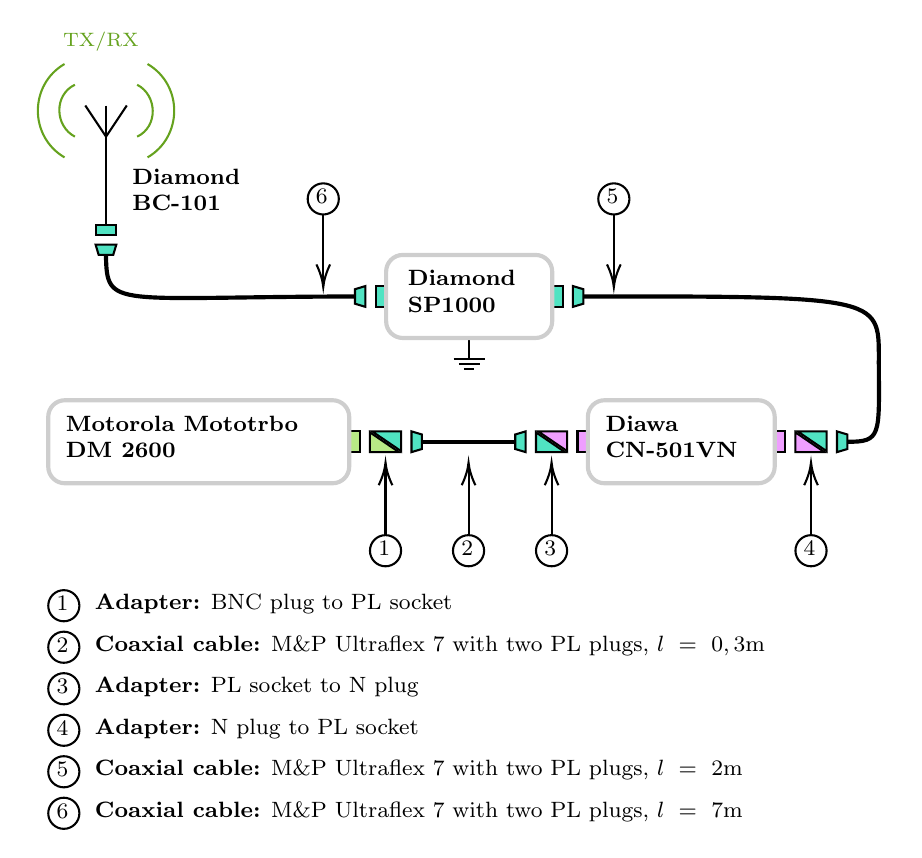
\begin{tikzpicture}[x=0.75pt,y=0.75pt,yscale=-1,xscale=1]
%uncomment if require: \path (0,479); %set diagram left start at 0, and has height of 479

%Straight Lines [id:da5218826641526857] 
\draw    (322.8,185) -- (322.8,195) ;
%Shape: Rectangle [id:dp3707976877259427] 
\draw  [fill={rgb, 255:red, 80; green, 227; blue, 194 }  ,fill opacity=1 ] (362.8,160) -- (367.8,160) -- (367.8,170) -- (362.8,170) -- cycle ;
%Shape: Rectangle [id:dp10664709959227037] 
\draw  [fill={rgb, 255:red, 80; green, 227; blue, 194 }  ,fill opacity=1 ] (277.8,160) -- (282.8,160) -- (282.8,170) -- (277.8,170) -- cycle ;
%Rounded Rect [id:dp527676076956175] 
\draw  [color={rgb, 255:red, 206; green, 206; blue, 206 }  ,draw opacity=1 ][line width=1.5]  (282.8,153) .. controls (282.8,148.58) and (286.38,145) .. (290.8,145) -- (354.8,145) .. controls (359.22,145) and (362.8,148.58) .. (362.8,153) -- (362.8,177) .. controls (362.8,181.42) and (359.22,185) .. (354.8,185) -- (290.8,185) .. controls (286.38,185) and (282.8,181.42) .. (282.8,177) -- cycle ;

%Straight Lines [id:da6289021026698145] 
\draw    (147.84,73) -- (147.84,133) ;
%Straight Lines [id:da47703805930667476] 
\draw    (137.84,73) -- (147.84,88) ;
%Straight Lines [id:da4218266835017126] 
\draw    (147.84,88) -- (157.84,73) ;
%Curve Lines [id:da5241031222048758] 
\draw [color={rgb, 255:red, 101; green, 162; blue, 30 }  ,draw opacity=1 ]   (162.84,63) .. controls (172.56,68) and (173.13,83.14) .. (162.84,88) ;
%Curve Lines [id:da3821737885384662] 
\draw [color={rgb, 255:red, 101; green, 162; blue, 30 }  ,draw opacity=1 ]   (167.84,53) .. controls (185.09,63.13) and (184.84,88.13) .. (167.84,98) ;

%Curve Lines [id:da3538255270661379] 
\draw [color={rgb, 255:red, 101; green, 162; blue, 30 }  ,draw opacity=1 ]   (132.84,88) .. controls (123.13,83) and (122.56,67.86) .. (132.84,63) ;
%Curve Lines [id:da889352578619292] 
\draw [color={rgb, 255:red, 101; green, 162; blue, 30 }  ,draw opacity=1 ]   (127.84,98) .. controls (110.59,87.88) and (110.84,62.87) .. (127.84,53) ;

%Shape: Rectangle [id:dp9150249297100126] 
\draw  [fill={rgb, 255:red, 80; green, 227; blue, 194 }  ,fill opacity=1 ] (142.84,130.5) -- (152.84,130.5) -- (152.84,135.5) -- (142.84,135.5) -- cycle ;
%Shape: Trapezoid [id:dp6261372647556653] 
\draw  [fill={rgb, 255:red, 80; green, 227; blue, 194 }  ,fill opacity=1 ][line width=0.75]  (152.8,140) -- (151.3,145) -- (144.3,145) -- (142.8,140) -- cycle ;
%Shape: Trapezoid [id:dp4286379946581531] 
\draw  [fill={rgb, 255:red, 80; green, 227; blue, 194 }  ,fill opacity=1 ][line width=0.75]  (272.8,170) -- (267.8,168.5) -- (267.8,161.5) -- (272.8,160) -- cycle ;
%Curve Lines [id:da8045163154695201] 
\draw [line width=1.5]    (147.8,145) .. controls (148.3,171.25) and (150.3,165.25) .. (267.8,165) ;
%Straight Lines [id:da19181563997268603] 
\draw    (315.3,195) -- (330.3,195) ;
%Straight Lines [id:da020619477423114985] 
\draw    (317.8,197.5) -- (327.8,197.5) ;
%Straight Lines [id:da9009961872255909] 
\draw    (320.3,200) -- (325.3,200) ;
%Shape: Rectangle [id:dp35598711466417887] 
\draw  [fill={rgb, 255:red, 239; green, 158; blue, 255 }  ,fill opacity=1 ] (470,230) -- (475,230) -- (475,240) -- (470,240) -- cycle ;
%Shape: Rectangle [id:dp4791882432942969] 
\draw  [fill={rgb, 255:red, 239; green, 158; blue, 255 }  ,fill opacity=1 ] (375,230) -- (380,230) -- (380,240) -- (375,240) -- cycle ;
%Shape: Rectangle [id:dp2776872187237942] 
\draw  [fill={rgb, 255:red, 184; green, 233; blue, 134 }  ,fill opacity=1 ] (265,230) -- (270,230) -- (270,240) -- (265,240) -- cycle ;
%Rounded Rect [id:dp5113702121898573] 
\draw  [color={rgb, 255:red, 206; green, 206; blue, 206 }  ,draw opacity=1 ][line width=1.5]  (120,223) .. controls (120,218.58) and (123.58,215) .. (128,215) -- (257,215) .. controls (261.42,215) and (265,218.58) .. (265,223) -- (265,247) .. controls (265,251.42) and (261.42,255) .. (257,255) -- (128,255) .. controls (123.58,255) and (120,251.42) .. (120,247) -- cycle ;

%Straight Lines [id:da5653713287945248] 
\draw [line width=1.5]    (300,235) -- (345,235) ;
%Shape: Trapezoid [id:dp6827000741886373] 
\draw  [fill={rgb, 255:red, 80; green, 227; blue, 194 }  ,fill opacity=1 ][line width=0.75]  (295,230) -- (300,231.5) -- (300,238.5) -- (295,240) -- cycle ;
%Shape: Trapezoid [id:dp5551727639514186] 
\draw  [fill={rgb, 255:red, 80; green, 227; blue, 194 }  ,fill opacity=1 ][line width=0.75]  (350,240) -- (345,238.5) -- (345,231.5) -- (350,230) -- cycle ;

%Shape: Right Triangle [id:dp6567087371846239] 
\draw  [fill={rgb, 255:red, 184; green, 233; blue, 134 }  ,fill opacity=1 ] (275,230.48) -- (288.98,240) -- (275,240) -- cycle ;
%Shape: Right Triangle [id:dp6439631638146213] 
\draw  [fill={rgb, 255:red, 80; green, 227; blue, 194 }  ,fill opacity=1 ] (290,239.52) -- (276.02,230) -- (290,230) -- cycle ;

%Shape: Right Triangle [id:dp7065836348516847] 
\draw  [fill={rgb, 255:red, 80; green, 227; blue, 194 }  ,fill opacity=1 ] (355,230.48) -- (368.98,240) -- (355,240) -- cycle ;
%Shape: Right Triangle [id:dp6791715198368578] 
\draw  [fill={rgb, 255:red, 239; green, 158; blue, 255 }  ,fill opacity=1 ] (370,239.52) -- (356.02,230) -- (370,230) -- cycle ;

%Rounded Rect [id:dp5242124209678602] 
\draw  [color={rgb, 255:red, 206; green, 206; blue, 206 }  ,draw opacity=1 ][line width=1.5]  (380,223) .. controls (380,218.58) and (383.58,215) .. (388,215) -- (462,215) .. controls (466.42,215) and (470,218.58) .. (470,223) -- (470,247) .. controls (470,251.42) and (466.42,255) .. (462,255) -- (388,255) .. controls (383.58,255) and (380,251.42) .. (380,247) -- cycle ;
%Shape: Right Triangle [id:dp9024696438630258] 
\draw  [fill={rgb, 255:red, 80; green, 227; blue, 194 }  ,fill opacity=1 ] (495,239.52) -- (481.02,230) -- (495,230) -- cycle ;
%Shape: Right Triangle [id:dp3027647623967811] 
\draw  [fill={rgb, 255:red, 239; green, 158; blue, 255 }  ,fill opacity=1 ] (480,230.48) -- (493.98,240) -- (480,240) -- cycle ;

%Curve Lines [id:da5556976336058517] 
\draw [line width=1.5]    (375.3,165) .. controls (526.33,164.83) and (520,165.25) .. (520.17,198.54) .. controls (520.34,231.82) and (521.33,235.17) .. (505,235) ;
%Shape: Trapezoid [id:dp7689909076073862] 
\draw  [fill={rgb, 255:red, 80; green, 227; blue, 194 }  ,fill opacity=1 ][line width=0.75]  (372.8,160) -- (377.8,161.5) -- (377.8,168.5) -- (372.8,170) -- cycle ;
%Shape: Trapezoid [id:dp5759023250736097] 
\draw  [fill={rgb, 255:red, 80; green, 227; blue, 194 }  ,fill opacity=1 ][line width=0.75]  (500,230) -- (505,231.5) -- (505,238.5) -- (500,240) -- cycle ;
%Straight Lines [id:da0668317935629783] 
\draw    (282.5,280) -- (282.5,247) ;
\draw [shift={(282.5,245)}, rotate = 450] [color={rgb, 255:red, 0; green, 0; blue, 0 }  ][line width=0.75]    (10.93,-3.29) .. controls (6.95,-1.4) and (3.31,-0.3) .. (0,0) .. controls (3.31,0.3) and (6.95,1.4) .. (10.93,3.29)   ;
%Shape: Circle [id:dp8618966688089644] 
\draw   (275,287.5) .. controls (275,283.36) and (278.36,280) .. (282.5,280) .. controls (286.64,280) and (290,283.36) .. (290,287.5) .. controls (290,291.64) and (286.64,295) .. (282.5,295) .. controls (278.36,295) and (275,291.64) .. (275,287.5) -- cycle ;


%Shape: Circle [id:dp06491171475414959] 
\draw   (315,287.5) .. controls (315,283.36) and (318.36,280) .. (322.5,280) .. controls (326.64,280) and (330,283.36) .. (330,287.5) .. controls (330,291.64) and (326.64,295) .. (322.5,295) .. controls (318.36,295) and (315,291.64) .. (315,287.5) -- cycle ;

%Straight Lines [id:da006440625484793738] 
\draw    (322.5,280) -- (322.5,247) ;
\draw [shift={(322.5,245)}, rotate = 450] [color={rgb, 255:red, 0; green, 0; blue, 0 }  ][line width=0.75]    (10.93,-3.29) .. controls (6.95,-1.4) and (3.31,-0.3) .. (0,0) .. controls (3.31,0.3) and (6.95,1.4) .. (10.93,3.29)   ;

%Shape: Circle [id:dp9167743181241499] 
\draw   (355,287.5) .. controls (355,283.36) and (358.36,280) .. (362.5,280) .. controls (366.64,280) and (370,283.36) .. (370,287.5) .. controls (370,291.64) and (366.64,295) .. (362.5,295) .. controls (358.36,295) and (355,291.64) .. (355,287.5) -- cycle ;

%Straight Lines [id:da48094261953448303] 
\draw    (362.5,280) -- (362.5,247) ;
\draw [shift={(362.5,245)}, rotate = 450] [color={rgb, 255:red, 0; green, 0; blue, 0 }  ][line width=0.75]    (10.93,-3.29) .. controls (6.95,-1.4) and (3.31,-0.3) .. (0,0) .. controls (3.31,0.3) and (6.95,1.4) .. (10.93,3.29)   ;

%Shape: Circle [id:dp1939511278206627] 
\draw   (480,287.5) .. controls (480,283.36) and (483.36,280) .. (487.5,280) .. controls (491.64,280) and (495,283.36) .. (495,287.5) .. controls (495,291.64) and (491.64,295) .. (487.5,295) .. controls (483.36,295) and (480,291.64) .. (480,287.5) -- cycle ;

%Straight Lines [id:da3351576985038338] 
\draw    (487.5,280) -- (487.5,247) ;
\draw [shift={(487.5,245)}, rotate = 450] [color={rgb, 255:red, 0; green, 0; blue, 0 }  ][line width=0.75]    (10.93,-3.29) .. controls (6.95,-1.4) and (3.31,-0.3) .. (0,0) .. controls (3.31,0.3) and (6.95,1.4) .. (10.93,3.29)   ;

%Shape: Circle [id:dp5129779571773962] 
\draw   (385,118) .. controls (385,113.86) and (388.36,110.5) .. (392.5,110.5) .. controls (396.64,110.5) and (400,113.86) .. (400,118) .. controls (400,122.14) and (396.64,125.5) .. (392.5,125.5) .. controls (388.36,125.5) and (385,122.14) .. (385,118) -- cycle ;

%Straight Lines [id:da6621400269321598] 
\draw    (392.5,158.5) -- (392.5,125.5) ;
\draw [shift={(392.5,160.5)}, rotate = 270] [color={rgb, 255:red, 0; green, 0; blue, 0 }  ][line width=0.75]    (10.93,-3.29) .. controls (6.95,-1.4) and (3.31,-0.3) .. (0,0) .. controls (3.31,0.3) and (6.95,1.4) .. (10.93,3.29)   ;

%Shape: Circle [id:dp7977203271441822] 
\draw   (245,118) .. controls (245,113.86) and (248.36,110.5) .. (252.5,110.5) .. controls (256.64,110.5) and (260,113.86) .. (260,118) .. controls (260,122.14) and (256.64,125.5) .. (252.5,125.5) .. controls (248.36,125.5) and (245,122.14) .. (245,118) -- cycle ;

%Straight Lines [id:da2162256591147207] 
\draw    (252.5,158.5) -- (252.5,125.5) ;
\draw [shift={(252.5,160.5)}, rotate = 270] [color={rgb, 255:red, 0; green, 0; blue, 0 }  ][line width=0.75]    (10.93,-3.29) .. controls (6.95,-1.4) and (3.31,-0.3) .. (0,0) .. controls (3.31,0.3) and (6.95,1.4) .. (10.93,3.29)   ;

%Shape: Circle [id:dp24834021243597504] 
\draw   (120,314) .. controls (120,309.86) and (123.36,306.5) .. (127.5,306.5) .. controls (131.64,306.5) and (135,309.86) .. (135,314) .. controls (135,318.14) and (131.64,321.5) .. (127.5,321.5) .. controls (123.36,321.5) and (120,318.14) .. (120,314) -- cycle ;

%Shape: Circle [id:dp7233992369838149] 
\draw   (120,334) .. controls (120,329.86) and (123.36,326.5) .. (127.5,326.5) .. controls (131.64,326.5) and (135,329.86) .. (135,334) .. controls (135,338.14) and (131.64,341.5) .. (127.5,341.5) .. controls (123.36,341.5) and (120,338.14) .. (120,334) -- cycle ;

%Shape: Circle [id:dp6313697664795326] 
\draw   (120,354) .. controls (120,349.86) and (123.36,346.5) .. (127.5,346.5) .. controls (131.64,346.5) and (135,349.86) .. (135,354) .. controls (135,358.14) and (131.64,361.5) .. (127.5,361.5) .. controls (123.36,361.5) and (120,358.14) .. (120,354) -- cycle ;

%Shape: Circle [id:dp03435814103609336] 
\draw   (120,374) .. controls (120,369.86) and (123.36,366.5) .. (127.5,366.5) .. controls (131.64,366.5) and (135,369.86) .. (135,374) .. controls (135,378.14) and (131.64,381.5) .. (127.5,381.5) .. controls (123.36,381.5) and (120,378.14) .. (120,374) -- cycle ;

%Shape: Circle [id:dp003390866078124999] 
\draw   (120,394) .. controls (120,389.86) and (123.36,386.5) .. (127.5,386.5) .. controls (131.64,386.5) and (135,389.86) .. (135,394) .. controls (135,398.14) and (131.64,401.5) .. (127.5,401.5) .. controls (123.36,401.5) and (120,398.14) .. (120,394) -- cycle ;

%Shape: Circle [id:dp7433181145978278] 
\draw   (120,414) .. controls (120,409.86) and (123.36,406.5) .. (127.5,406.5) .. controls (131.64,406.5) and (135,409.86) .. (135,414) .. controls (135,418.14) and (131.64,421.5) .. (127.5,421.5) .. controls (123.36,421.5) and (120,418.14) .. (120,414) -- cycle ;



% Text Node
\draw (159,102) node [anchor=north west][inner sep=0.75pt]  [font=\footnotesize] [align=left] {\textbf{Diamond }\\\textbf{BC-101}};
% Text Node
\draw (127,221) node [anchor=north west][inner sep=0.75pt]  [font=\footnotesize] [align=left] {\textbf{Motorola Mototrbo}\\\textbf{DM 2600}};
% Text Node
\draw (387,221) node [anchor=north west][inner sep=0.75pt]  [font=\footnotesize] [align=left] {\textbf{Diawa}\\\textbf{CN-501VN}};
% Text Node
\draw (291.8,151) node [anchor=north west][inner sep=0.75pt]  [font=\footnotesize] [align=left] {\textbf{Diamond}\\\textbf{SP1000}};
% Text Node
\draw (125.69,36) node [anchor=north west][inner sep=0.75pt]  [font=\scriptsize,color={rgb, 255:red, 101; green, 162; blue, 30 }  ,opacity=1 ] [align=left] {TX/RX};
% Text Node
\draw (277.5,281.5) node [anchor=north west][inner sep=0.75pt]  [font=\footnotesize] [align=left] {1};
% Text Node
\draw (317.5,281.5) node [anchor=north west][inner sep=0.75pt]  [font=\footnotesize] [align=left] {2};
% Text Node
\draw (357.5,281.5) node [anchor=north west][inner sep=0.75pt]  [font=\footnotesize] [align=left] {3};
% Text Node
\draw (482.5,281.5) node [anchor=north west][inner sep=0.75pt]  [font=\footnotesize] [align=left] {4};
% Text Node
\draw (387.5,112) node [anchor=north west][inner sep=0.75pt]  [font=\footnotesize] [align=left] {5};
% Text Node
\draw (247.5,112) node [anchor=north west][inner sep=0.75pt]  [font=\footnotesize] [align=left] {6};
% Text Node
\draw (122.5,308) node [anchor=north west][inner sep=0.75pt]  [font=\footnotesize] [align=left] {1};
% Text Node
\draw (122.5,328) node [anchor=north west][inner sep=0.75pt]  [font=\footnotesize] [align=left] {2};
% Text Node
\draw (122.5,348) node [anchor=north west][inner sep=0.75pt]  [font=\footnotesize] [align=left] {3};
% Text Node
\draw (122.5,368) node [anchor=north west][inner sep=0.75pt]  [font=\footnotesize] [align=left] {4};
% Text Node
\draw (122.5,388) node [anchor=north west][inner sep=0.75pt]  [font=\footnotesize] [align=left] {5};
% Text Node
\draw (122.5,408) node [anchor=north west][inner sep=0.75pt]  [font=\footnotesize] [align=left] {6};
% Text Node
\draw (141,307) node [anchor=north west][inner sep=0.75pt]  [font=\footnotesize] [align=left] {\textbf{Adapter:} BNC plug to PL socket};
% Text Node
\draw (141,327) node [anchor=north west][inner sep=0.75pt]  [font=\footnotesize] [align=left] {\textbf{Coaxial cable:} M\&P Ultraflex 7 with two PL plugs, $\displaystyle l\ =\ 0,3\mathrm{m}$};
% Text Node
\draw (141,347) node [anchor=north west][inner sep=0.75pt]  [font=\footnotesize] [align=left] {\textbf{Adapter:} PL socket to N plug};
% Text Node
\draw (141,367) node [anchor=north west][inner sep=0.75pt]  [font=\footnotesize] [align=left] {\textbf{Adapter:} N plug to PL socket};
% Text Node
\draw (141,387) node [anchor=north west][inner sep=0.75pt]  [font=\footnotesize] [align=left] {\textbf{Coaxial cable:} M\&P Ultraflex 7 with two PL plugs, $\displaystyle l\ =\ 2\mathrm{m}$};
% Text Node
\draw (141,407) node [anchor=north west][inner sep=0.75pt]  [font=\footnotesize] [align=left] {\textbf{Coaxial cable:} M\&P Ultraflex 7 with two PL plugs, $\displaystyle l\ =\ 7\mathrm{m}$};


\end{tikzpicture}

	\caption{Schematic structure of the base station radio infrastructure.}
	\label{fig:tikz_base_camp_radio}
\end{figure}
Figure \ref{fig:tikz_base_camp_radio} provides an illustration. There are gaps between the devices and components to make the schematic structure easier to read.\footnote{In practice these are connected.} Green connectors represent a BNC plug or socket, turquoise connectors represent a PL plug or socket and pink connectors represent a N plug or socket. For more information on whether it is a socket or a plug, see figure \ref{fig:tikz_base_camp_radio} and tables \ref{tab:table_dm2600_specs} through \ref{tab:table_ultraflex_7_specs}. Adapters -- such as \circled{\footnotesize{1}} and \circled{\footnotesize{3}} -- are characterized by a rectangle with a diagonal drawn in. The colors in the resulting right-angled triangles indicate which connectors an adapter has. Coaxial cables are drawn with a thicker line and trapezoids as connectors -- for example \circled{\footnotesize{2}}, \circled{\footnotesize{5}} and \circled{\footnotesize{6}}. Because the coaxial cables were delivered without connectors, they were installed afterwards. The connectors of the DM 2600, Diawa CN-501VN, Diamond SP1000 and Diamond BC-101 are marked by a small rectangle which is in direct contact with the associated device or component. These have factory-installed connectors which their data sheets already take into account.

From the data sheet of the DM 2600, from which an excerpt is provided in table \ref{tab:table_dm2600_specs}, it can be seen that its maximum transmission power is $25\mathrm{W}$ and its sensitivity -- in the worst case -- is $0,25\mathrm{\mu V}$.
\begin{table}[h!]
	\centering
	\footnotesize
\begin{tabular}{|l|c|}
	\hline
	\multicolumn{2}{|c|}{\textbf{Motorola Mototrbo DM 2600 (VHF digital) specifications}} \\
	\hline
 	Frequency & $136\mathrm{MHz}$ to $174\mathrm{MHz}$ \\
	System impedance & $50\Omega$\\
 	Dimensions $\mathrm{(H \times W \times D)}$ & $44 \times 169 \times 134 \mathrm{mm}$ \\%
 	Mass & $1,3\mathrm{kg}$ \\%
	Power supply & $13,2\mathrm{VDC}$ (nominal) ($10,8$ to $15,6\mathrm{VDC}$) \\
	Current standby & $0,81\mathrm{A}$ (max.) \\
	Current RX & $2\mathrm{A}$ (max.) \\
	Current TX & $11\mathrm{A}$ (max.) \\
	Operating temperature & $-30^\circ \mathrm{C}$ to $60^\circ \mathrm{C}$ \\
	Storage temperature & $-40^\circ \mathrm{C}$ to $85^\circ \mathrm{C}$ \\
	RX sensitivity 5\% BER: & $0,25\mathrm{\mu V}$ ($0,19\mathrm{\mu V}$ typical) \\
	TX power output & $1\mathrm{W}$ to $25\mathrm{W}$ \\
	Connector & BNC socket\\
	\hline
\end{tabular}
	\caption{Excerpt from the data sheet of the Motorola Mototrbo DM 2600 mobile radio. \cite{DM2600:2013}}
	\label{tab:table_dm2600_specs}
\end{table}
Its maximum transmission and minimum required reception power therefore follow to:
\begin{equation} \label{eq:power_BSt_tx}
	\centering
	P_\mathrm{T,dBW} =  10\mathrm{dBW} \cdot \log_{10} \left( \dfrac{25\mathrm{W}}{1\mathrm{W}} \right) = 13,979\mathrm{dBW}\text{,}
\end{equation}
\begin{equation} \label{eq:power_BSt_min}
	\centering
	P_\mathrm{min,dBW} = 10\mathrm{dBW} \cdot \log_{10} \left( \dfrac{\left(0,25\cdot10^{-6}\mathrm{V}\right)^2}{50\Omega} \right) = -149,031\mathrm{dBW}\text{.}
\end{equation}

It is assumed that the CN-501VN will not cause any loss or gain in the antenna feed line as its data sheet does not contain any specifications on this matter. An excerpt of said data sheet can be seen in the table \ref{tab:table_daiwa_cn_501}.
\begin{table}[h!]
	\centering
	\footnotesize
\begin{tabular}{|l|c|}
	\hline
	\multicolumn{2}{|c|}{\textbf{Daiwa CN-501VN specifications}} \\
	\hline
 	Frequency & $140\mathrm{MHz}$ to $525\mathrm{MHz}$ \\
	Input/Output impedance & $50\Omega$\\
	Dimensions $\mathrm{(H \times W \times D)}$ & $80 \times 155 \times 100 \mathrm{mm}$ \\%
 	Weight& $0,67\mathrm{kg}$ \\%
	Power range & $20\mathrm{W}/200\mathrm{W}$ (forward) \\
	Power rating & $200\mathrm{W}$ ($140\mathrm{MHz}$ to $525\mathrm{MHz}$) \\
	Tolerance & $\pm10\%$ at full scale \\
	VSWR measurement range & $1$ to $\infty$\\
	VSWR detection sensitivity & $200\mathrm{W}$ (min.)\\
	Connector & $2 \times \text{N socket}$ \\
	\hline
\end{tabular}
	\caption{Excerpt from the data sheet of the Daiwa CN-501VN cross needle VSWR \& power meter.\cite{Daiwa-industry-co.:2016}}
	\label{tab:table_daiwa_cn_501}
\end{table}

The SP1000 has an insertion loss of less than $0,2\mathrm{dB}$ and a VSWR of less than $1,2$ as shown in the table \ref{tab:table_lightning_arrestor_specs}.
\begin{table}[h!]
	\centering
	\footnotesize
\begin{tabular}{|l|c|}
	\hline
	\multicolumn{2}{|c|}{\textbf{Diamond SP1000 specification}} \\
	\hline
 	Frequency range & \numrange{0}{1000}$\mathrm{MHz}$ \\ % DC -> 0Hz 
 	Impedance & $50\Omega$ \\
 	VSWR & $< 1,2$ \\
	Insertion loss & $< 0,2\mathrm{dB}$ \\
 	Max. power rating & $400\mathrm{W}$ \\
	Impulse wave discharge voltage & $1000\mathrm{V}$ \\
	Impulse wave discharge current & $6000\mathrm{A}$ \\
	Impulse wave retention voltage & $350\mathrm{VDC} \pm 20\%$ \\
	Insulating resistance ($100\mathrm{VDC}$) & $> 10000\mathrm{M}\Omega$ \\
	Connector & $2 \times \text{PL socket}$ \\
	\hline
\end{tabular}
	\caption{Excerpt from the data sheet of the Diamond SP1000 lightning arrester. \cite{SP1000:2020}}
	\label{tab:table_lightning_arrestor_specs}
\end{table}
If now the worst case is assumed -- which means that the insertion loss is exactly $0,2\mathrm{dB}$ and the VSWR is exactly $1,2$ -- then the total loss caused by this component is the sum of the insertion and the mismatch loss:
\begin{equation} \label{eq:losses_BSt_arr}
	\centering
	L_\mathrm{arr,dB} = 0,2\mathrm{dB} - 10\mathrm{dB} \cdot \log_{10} \left(1 - \left(\dfrac{1,2 - 1}{1,2 + 1}\right)^2\right) = 0,236\mathrm{dB}\text{.}
\end{equation}

As can be seen in the table \ref{tab:table_bc101_specs}, the BC-101 has a gain of $G_\mathrm{ant,dBi} = 3,5\mathrm{dBi}$ and a VSWR of less than $1,5$.
\begin{table}[h!]
	\centering
	\footnotesize
\begin{tabular}{|l|c|}
	\hline
	\multicolumn{2}{|c|}{\textbf{Diamond BC-101 specifications}} \\
	\hline
 	Type & 5/8 wave ground plane \\
 	Frequency & $144\mathrm{MHz}$ to $174\mathrm{MHz}$ \\
	Impedance & $50\Omega$\\
	Gain & $3,5\mathrm{dBi}$\\
 	Power rating & $200\mathrm{W}$ (max.) \\
 	VSWR & $< 1,5$ \\
	Weight & $0,86\mathrm{kg}$ \\
	Connector & PL plug \\
	\hline
\end{tabular}
	\caption{Excerpt from the data sheet of the Diamond BC-101 VHF fixed station antenna.\cite{antenna:2020}}
	\label{tab:table_bc101_specs}
\end{table}
With $\mathrm{VSWR} = 1,5$, the mismatch loss in the worst case can be calculated as shown in the equation (\ref{eq:losses_BSt_ant}).
\begin{equation} \label{eq:losses_BSt_ant}
	\centering
	L_\mathrm{ant,dB} = - 10\mathrm{dB} \cdot \log_{10} \left(1 - \left(\dfrac{1,5 - 1}{1,5 + 1}\right)^2\right) = 0,177\mathrm{dB}
\end{equation}
Regarding this antenna, it should also be mentioned that a mast will be made available at the mission site. Therefore, the height of the mast can vary from mission to mission. An antenna, which is set up on a $1\mathrm{m}$ high tripod on a freight container in accordance with ISO 668, has approximately a height of $h _\mathrm{BSt} = 3,6\mathrm{m}$ above the ground. This height is used for the link budget estimation. 

All coaxial cables used for the voice communication system are Messi \& Paoloni Ultraflex 7 coaxial cables. An excerpt of the data sheet of this coaxial cable can be found in the table \ref{tab:table_ultraflex_7_specs} and the attenuation as a function of the frequency -- interpolated with a \MATLAB program -- according to its data sheet, in the figure \ref{fig:image_attenuation_UF7}. 
\begin{table}[h!]
	\centering
	\footnotesize
\begin{tabular}{|l|c|}
	\hline
	\multicolumn{2}{|c|}{\textbf{Messi \& Paoloni Ultraflex 7 specifications}} \\
	\hline
 	Frequency & $1,8\mathrm{MHz}$ to $8000\mathrm{MHz}$ \\
	Impedance & $50\pm3\Omega$ (at $200\mathrm{MHz}$)\\
	Operating temperature & $-40^\circ \mathrm{C}$ to $60^\circ \mathrm{C}$ \\
	Inner conductor resistance & $7,3\Omega\mathrm{km}^{-1}$ \\
	Outer conductor resistance & $9,8\Omega\mathrm{km}^{-1}$ \\
	Capacitance & $75\pm3\mathrm{pFm}^{-1}$ \\
	Power rating & $8000\mathrm{W}$ (peak) \\
	Net. weight & $6,9\mathrm{kg}/100\mathrm{m}$ \\
	Connector & none \\
	\hline
\end{tabular}
	\caption{Excerpt from the data sheet of the Messi \& Poloni Ultraflex 7 coaxial cable. \cite{Paoloni:2021}}
	\label{tab:table_ultraflex_7_specs}
\end{table}
\begin{figure}[h!]
	\centering
  	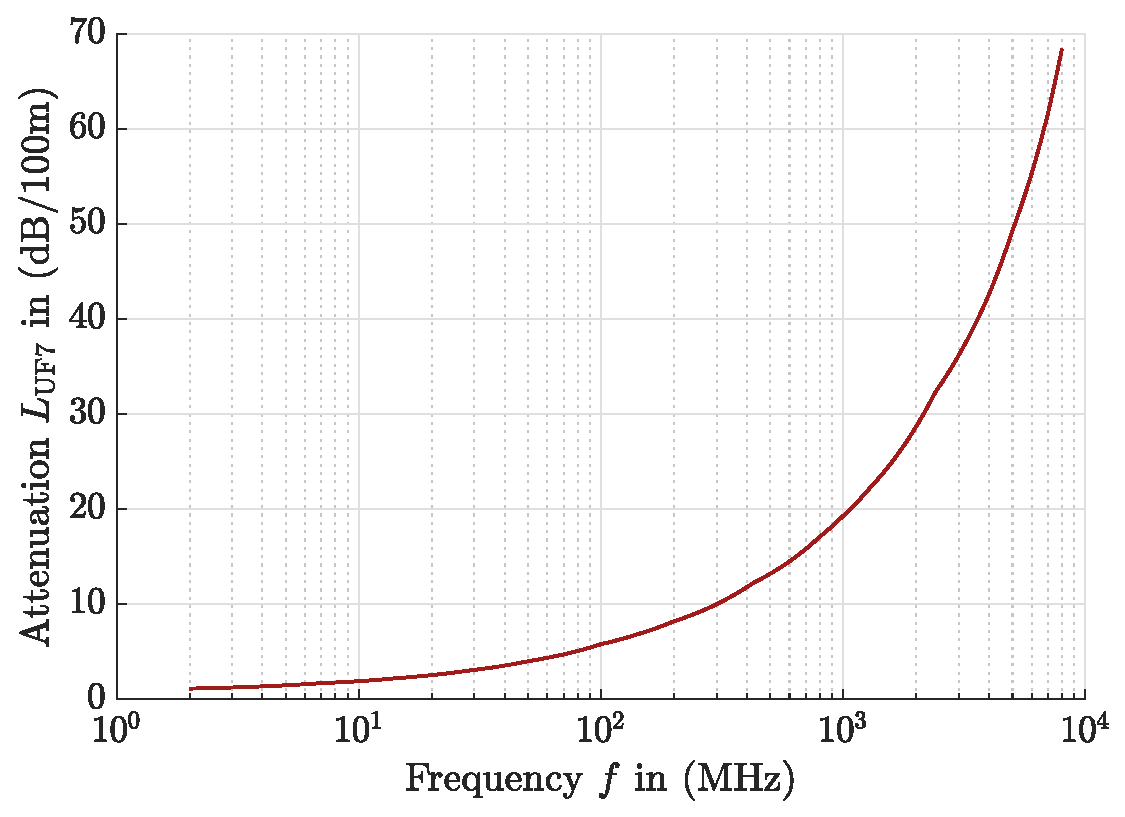
\includegraphics[width = 0.67\textwidth]{image_attenuation_UF7.eps}
  	\caption{Attenuation of the Messi \& Paoloni Ultraflex 7 coaxial cable for $20^\circ \mathrm{C}$. For the frequency $f_\sim = 158,950\mathrm{MHz}$, the attenuation is around $7,2471\mathrm{dB/100m}$. (Recreated from: \cite{Paoloni:2021})}
	\label{fig:image_attenuation_UF7}
\end{figure}
Based on this, an attenuation of $7,2471\mathrm{dB/100m}$ was determined for the frequency $f_\sim = 158,950\mathrm{MHz}$. The cable lengths of the individual coaxial cables in the systems can be taken from the figure \ref{fig:tikz_base_camp_radio}. This results in an insertion loss -- without connectors -- of:
\begin{equation} \label{eq:losses_BSt_coax}
	\centering
	L_\mathrm{coax,dB} = \dfrac{7,2471 \cdot 9,3}{100}\mathrm{dB} = 0,674\mathrm{dB}\text{.}
\end{equation}
It is noted, that $L_\mathrm{coax,dB}$ increases as the cable length increases. It can become significantly greater if the antenna is mounted at a location further away from the base station. 

Regarding the attenuation of the numbered adapters and connectors, which also includes the connectors of the coaxial cables in the figure \ref{fig:tikz_base_camp_radio}, it is assumed that each of these has an attenuation of $0,1 \mathrm{dB}$ \cite{LinkMargin:2016}. With $N_\mathrm{I} = 9$, the total insertion loss caused by the connectors and adapters follows to:
\begin{equation} \label{eq:losses_BSt_conn}
	\centering
	L_\mathrm{conn/adapt,dB} = 0,9\mathrm{dB}\text{.}
\end{equation}
An assumption was made because no data sheets for the adapters and connectors were found. 

From the above, the total loss of the antenna feed line now results in:
\begin{equation} \label{eq:losses_BSt}
	\centering
	L_\mathrm{BSt,dB} = L_\mathrm{arr,dB} + L_\mathrm{ant,dB} + L_\mathrm{coax,dB} + L_\mathrm{conn/adapt,dB} = 1,987\mathrm{dB}\text{.}
\end{equation}








%\textcolor{rgb, 255:red, 80; green, 227; blue, 194 }{turquoise} 



